% Chapter 3
\chapter{ZigBee network: Waspmotes} % Main chapter title
\label{Chapter3} % For referencing the chapter elsewhere, use \ref{Chapter1} 
\lhead{Chapter 3. \emph{ZigBee network: Waspmotes}} % This is for the header on each page - perhaps a shortened title

%----------------------------------------------------------------------------------------
\section{Power considerations}
\subsection{Waspmote power modes}
The libelium Waspmote has 4 operational modes: ON, Sleep, Deep Sleep and Hibernate. They differ from which type of interruptions they can be woken up and duration interval. For our application we want sleep intervals of 30 seconds and more, so only Deep Sleep and Hibernate mode are of interest. Table \ref{tab:cons1} summarizes the Waspmotes operational modes.
\begin{table}[!ht]
\begin{center}
\begin{tabular}[!ht]{|c|c|c|c|c|}
\hline
\textbf{Mode} & \textbf{Consumption} & \textbf{CPU} & \textbf{Cycle} & \textbf{Accepted Interruptions}\\
\hline
ON & 9mA & ON & - & Synch and Asynch\\
\hline
Sleep & 62$\mu$A  & ON & 31ms - 8s & Synch (WDT) and Asynch\\
\hline
Deep Sleep & 62$\mu$A & ON & 8s - min/hours/days & Synch (RTC) and Asynch\\
\hline
Hibernate & 0.7$\mu$A & OFF & 8s - min/hours/days & Synch (RTC)\\
\hline
\end{tabular}
\caption{Operational modes of Libelium Waspmote V1.1}
\label{tab:cons1}
\end{center}
\end{table}
\subsubsection{Deep Sleep}
In deep sleep mode the main program is paused and the CPU passes to a latent state. Triggers are as well synchronous interruptions (RTC) as asynchronous interruptions. Examples of asynchronous interruptions are low battery level or a sensor that reaches a certain trigger value.\bigskip
\begin{figure}[ht]
\centering
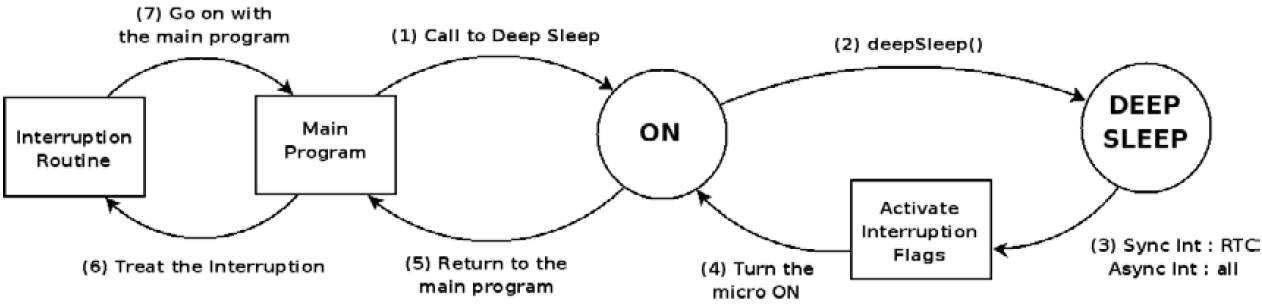
\includegraphics[height=3cm]{deepSleep}
\rule{30em}{0.5pt}
\caption{Waspmote going from ON to Deep Sleep}
\label{fig:deepSleep}
\end{figure}\bigskip
\\In figure \ref{fig:deepSleep} the process from going to operational mode ON to Deep Sleep is shown. The main advantage of this mode is that the program is only paused, so the program stack and thus all variable values keep their values. When the Waspmote is turned back on it simply executes the next instruction.
\subsubsection{Hibernate}
Hibernate mode consumes roughly 100 times less energy than Deep Sleep. This is made possible by disconnecting all the Waspmote's modules, including the microcontroller. The RTC gets his power through the auxiliary battery. So if hibernate mode stops working it is probably necessary to replace the Waspmote's button battery. Figure \ref{fig:hibernate} demonstrates the process from ON to hibernate. \\
\begin{figure}[ht]
\centering
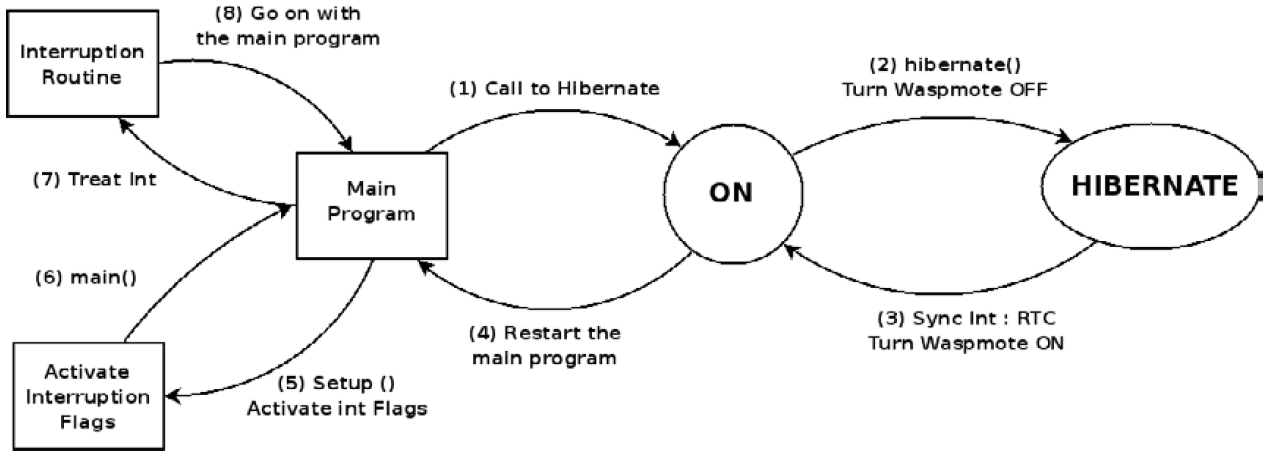
\includegraphics[height=4.5cm]{hibernate}
\rule{30em}{0.5pt}
\caption{Waspmote going from ON to Hibernate}
\label{fig:hibernate}
\end{figure}
This means the CPU is also switched of and does not remember any values from variables. When waking up the Waspmote reinitializes, the microprocessor is reset and the program restarts from the beginning. Both \textbf{setup} and \textbf{loop} routines are executed as if the main switch would be activated. By placing the \verb+ifHibernate()+ function in setup the program can determine if it came from a hardware reset or from a hibernate reset. To be able to wake up from hibernate mode the hibernate jumper must be removed correctly. See section .... for remarks on this issue. \\Because not all Libelium's API functions regarding hibernate in combination with the different alarm modes work, it is advised to use the functions provided in \textbf{WaspXBeeZBNode.h}. 
%----------------------------------------------------------------------------------------
\subsection{Sampling sensors}
To measure the sensors, originally we took 10 samples with 100 milliseconds recommended delay between the measurements and calculated the average. Since we want to make the energy consumption as low as possible we now do the iterations without delay. Appendix \ref{apendixSensorSensitivity} contains 60 test samples per sensor and indicates that there is no significant difference on the average by removing this delay. Except for CO$_{2}$ measurements, removing the delay saves about 1000 milliseconds per measured sensor.\\ 
Because the first sample often shows a slight deviation, the program takes 11 samples but bases the average on the last 10 values.
%-------------------------------------------
\subsection{Battery life estimation}
In order to be able to give recommended sensor measuring intervals this section will analyse the estimated battery life of the Waspmotes. Table \ref{tab:cons2} enumerates the most common components typical consumption.
\begin{table}[!ht]
\begin{center}
\begin{tabular}[!ht]{|c|c|}
\hline
\textbf{Action} & \textbf{Average Current}\\
\hline
XBee, sending, & 105mA\\
\hline
CO$_{2}$ & 50mA\\
\hline
XBee, ON & 45mA\\
\hline
Waspmote, ON & 9mA\\
\hline
Pressure & 7mA\\
\hline
Humidity & 380$\mu$A\\
\hline
Waspmote, sleep & 62$\mu$A\\
\hline
Temperature & 6$\mu$A\\
\hline
Waspmote, hibernate & 0,007$\mu$A\\
\hline
\end{tabular}
\caption{Operational modes of Libelium Waspmote V1.1}
\label{tab:cons2}
\end{center}
\end{table}
The batteries included with our Waspmotes are rechargeable Lithium-ion batteries with a capacity of 6600mAH. The Waspmote that will be deployed on the roof of Group T, campus Vesalius will also have a 12V solar panel with a charging current up to 280 mA to extend its battery life. The other batteries can by charged manually or by USB (5V, 100mA). Lithium-ion have a self-discharge rate of typcially 1 to 2 percent per month and since the used batteries are new we expect a high battery efficiency.\\
%-------------------------------------------
\subsubsection{XBee and Waspmote start-up times}
For the XBee node to join an existing network there are two power related possibilities. Either the Waspmote has been turned on already sufficiently long and the XBee had more than enough time to join the network, or either the XBee wasn't joined yet and the program needs to wait on this. From the experiments done at our apartment we came to following conclusions:
\begin{enumerate}
\item It takes about 2.5 seconds to join a network after powered on.
\item If the XBee is joined, the program still needs to confirm this. This takes 452 milliseconds.
\item The sending time is constant, about 158 ms, if the XBee had more than 2.5 seconds to join. However in case the XBee must send immediately after it is joined, the sending time is not constant and takes on average 611 milliseconds.
\item The sending time increases if there are more obstructions between the antennas. 
\end{enumerate}
With these characteristics we came to results discussed in the next sections. For the validation of these conclusions please see appendix \ref{AppendixA}. Table \ref{tab:sendTime} sums up the results of the distance-relation test.
\begin{table}[!ht]
\begin{center}
\begin{tabular}[!ht]{|c|c|}
\hline
\textbf{Distance} & \textbf{Average sending time (ms)}\\
\hline
Air & 158\\
\hline
1 Floor & 268\\
\hline
2 Floors & 357\\
\hline
3 Floors & 484\\
\hline
4 Floors & 558\\
\hline
5 Floors & unreachable\\
\hline
\end{tabular}
\caption{Distance consequence on send times}
\label{tab:sendTime}
\end{center}
\end{table}\\
To save power the Waspmote can store the values for a user determined time. Taking samples and save them to EEPROM in case of hibernate mode takes only 6 - 7\% of the time to measure and send. Table \ref{tab:sendTime3} confirms this.
\begin{table}[!ht]
\begin{center}
\begin{tabular}[!ht]{|c|c|}
\hline
\textbf{Nr of samples per sensor} & \textbf{Average ON time (ms)}\\
\hline
10 & 210\\
\hline
3 & 194\\
\hline
\end{tabular}
\caption{Time needed to sample and store 4 sensors}
\label{tab:sendTime3}
\end{center}
\end{table}
%-------------------------------------------
\subsubsection{Battery life with standard program optimizations}\label{batLife1}
The application scenario for this battery test is as follow: the Waspmote will be turned on as short as possible and 4 sensors, namely temperature, humidity, pressure and battery level will be sampled. The node will take 10 samples for each sensor and calculate the average. Those values are put into one ZigBee packet and sent to the gateway. By adapting the sleep time between the event we came to the rather disappointing results shown in figure \ref{fig:batCalcHP}.\\ The graph in figure \ref{fig:batCalcHP1} breaks down the total energy consumption to five categories. It shows the monthly energy consumption as a function of the time between the events. For small intervals the active energy usage is huge. Only starting at 20 minutes sleep time the self-discharge becomes dominant and from 3 hours on the sleep mode current also becomes dominant.\\
Since the Waspmotes use this much energy when applied this way we will call this the High Performance mode from now on. The next section calculates an alternative approach, referred to as Power Saver mode. This nomenclature is continued in the program:
\begin{alltt}
    typedef enum \{HIGHPERFORMANCE, POWERSAVER\} PowerPlan; 
\end{alltt}
\begin{figure}[htbp]
\centering
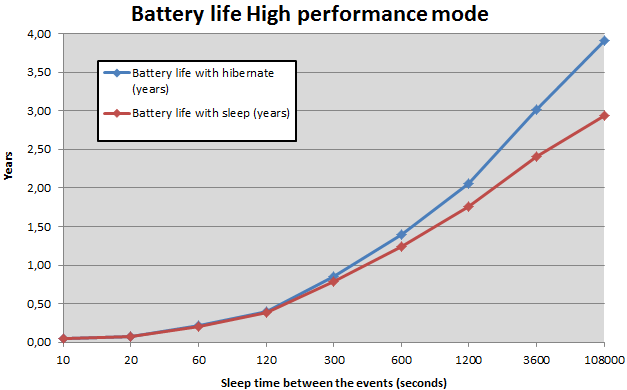
\includegraphics[height=8.5cm]{batCalcHP}
\rule{30em}{0.5pt}
\caption{Battery life in High performance mode}
\label{fig:batCalcHP}
\end{figure}
\begin{figure}[htbp]
\centering
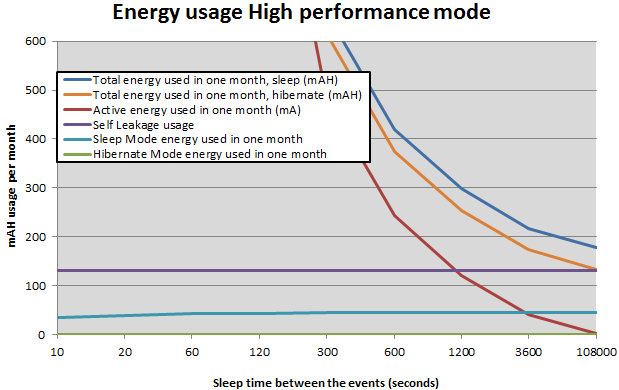
\includegraphics[height=8.5cm]{battery1}
\rule{30em}{0.5pt}
\caption{Energy usage in High performance mode}
\label{fig:batCalcHP1}
\end{figure}
Table \ref{tab:cons2} summarizes the battery duration in years of both performance and power saver mode.
\begin{table}[!ht]
\begin{center}
\begin{tabular}{cc|c||c|c|l}
\cline{2-5}
 & \multicolumn{2}{ |c|| }{Deep Sleep} & \multicolumn{2}{c}{Hibernate}\vline\\ \cline{1-5}
\multicolumn{1}{ |c| }{Sleep duration} & High Performance & Power Saver & High Performance & Power Saver    \\ \cline{1-5}
\multicolumn{1}{ |c| }{10s} & 0,05 & 0,92 & 0,05 & 1,00    \\ %\cline{1-5}
\hline
\multicolumn{1}{ |c| }{1min} & 0,21 & 2,15 & 0,21 & 2,63   \\ %\cline{1-5}
\hline
\multicolumn{1}{ |c| }{3min} & 0,79 & 2,75 & 0,85 & 3,59   \\ %\cline{1-5}
\hline
\multicolumn{1}{ |c| }{10min} & 1,25 & 2,85 & 1,39 & 3,76   \\ %\cline{1-5}
\hline
\multicolumn{1}{ |c| }{20min} & 1,75 & 2,90 & 2,06 & 3,85  \\ %\cline{1-5}
\hline
\multicolumn{1}{ |c| }{1h} & 2,41 & 2,94 &3,02 & 3,91    \\ %\cline{1-5}
\hline
\multicolumn{1}{ |c| }{3h} & 2,94 & 2,96 &3,90 & 3,94    \\ %\cline{1-5}
\hline
%\multicolumn{1}{ |c  }{\multirow{2}{*}{Powers} } &
%\multicolumn{1}{ |c| }{gcd} & 2 & 2 & 0 & 0 & min \\ \cline{2-6}
%\multicolumn{1}{ |c  }{}                        &
%\multicolumn{1}{ |c| }{lcm} & 3 & 3 & 1 & 1 & max \\ \cline{1-6}
\end{tabular}
\caption{Battery life in years for High Performance and Power Saver}
\label{tab:cons2}
\end{center}
\end{table}\\

%-------------------------------------------
\subsubsection{Battery life with extra optimizations}
As shown earlier in this section, sending values requires that the Waspmote is on for at least 3 seconds. In addition the XBee uses about five times the energy of the Waspmote. For end devices it is obviously recommended to turn on the XBee as little as possible, within a user defined limit.\\ Figure \ref{fig:batCalcPS} shows the same results as the application scenario discussed in section \ref{batLife1} and adds the results for a mode further referred to as Power Saver.\\
The implementation of this mode will depend on the nodes sleep settings. For \textit{Deep Sleep} the values can simply be stored on the heap, but for \textit{Hibernate} the values must be written to EEPROM.\\
Because of the size limit of a ZigBee packet we can store maximum 30 values and send them in one packet. However, if the sensor measuring interval is small the user can opt to store more values and send two or more packets after each other. The values for Power Saver in table \ref{tab:cons2} are of an example scenario that takes 60 measurements and then sends them in two packets to the gateway. It are also those results which are put in function of time in figure \ref{fig:batCalcPS}.  
\begin{figure}[htbp]
\centering
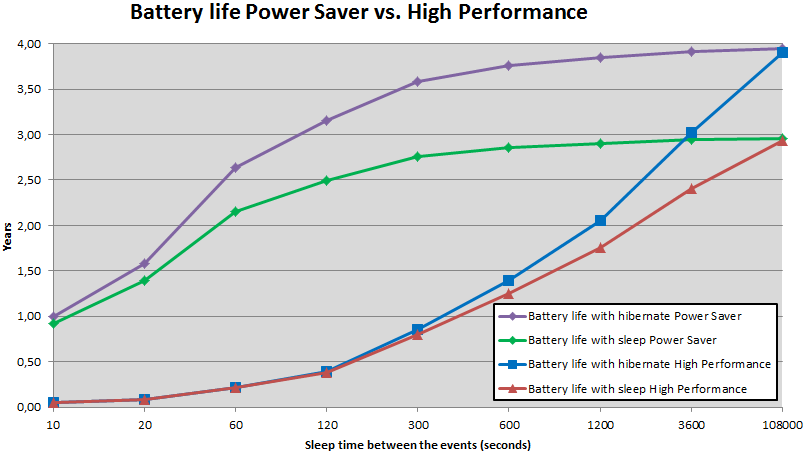
\includegraphics[height=8.5cm]{battery2}
\rule{30em}{0.5pt}
\caption{Battery life High Performance vs. Power Saver}
\label{fig:batCalcPS}
\end{figure}
\begin{figure}[htbp]
\centering
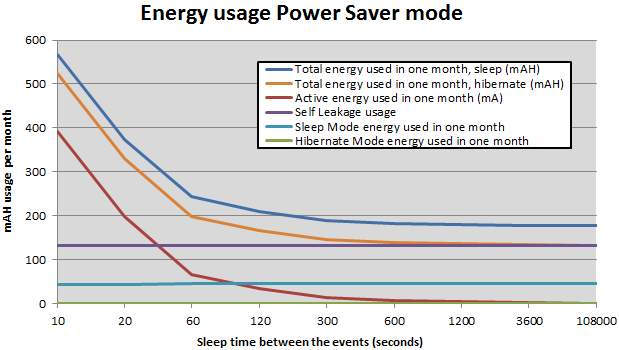
\includegraphics[height=8.5cm]{battery3}
\rule{30em}{0.5pt}
\caption{Energy usage in Power Saver mode}
\label{fig:batCalcPS1}
\end{figure}\\
As visible on figure \ref{fig:batCalcPS} \textit{Hibernate} has more influence in Power Saver mode, already extending battery life significantly at a 20 seconds interval comparing to a 10 minutes interval in High Performance mode. Also the energy breakdown graph in figure \ref{fig:batCalcPS1} shows that the interval times must be increased much less before the dominant factor is self-discharge and sleep mode energy consumption, compared to figure \ref{fig:batCalcHP1}.\\By reducing the sensor measurement accuracy battery life can be extended with modest 3 - 4\%, best case scenario. Please see appendix \ref{appendixA} for details.\\
In case the measuring intervals are small it is recommended to use \textit{Deep Sleep} instead of \textit{Hibernate}, since in hibernate the values are written to EEPROM. Equation \ref{eq:1} shows this can be very destructive for the Waspmote. Depending on how much freedom the user is given, the program can make the decision to switch to \textit{Deep Sleep} on itself, or the installation's administrator can control this.

  
\subsection{Device start-up}
Whether we come out of a hardware reset or a hibernate reset, the first thing the node will do is try to establish a connection with the network. Depending which reset we come from different routines will be executed. In normal operation mode this process only takes about 2 seconds (Please see appendix \ref{fig:envA} for more measurement results). However, when a node is not able to join a network it will go into panic mode. This means that if the operating sleeping time is small, this time will be ignored and the node will wake up less frequently until it is able to rejoin the network, that way saving battery power. Supposing the node is able to rejoin the network, it will send the number of panics it experienced to the coordinator so a network administrator can investigate of the severity of the problem.

\subsubsection{Full initialization}
When the program is executed for the first time or when a hardware reset is detected the XBee will execute a full initialization process and the RTC will be set to zero. This means the default PAN ID and possibly other user settings like node ID will be written to the XBee. After this write the XBee must be re-setted (turn the power off and back on) and only than the joining attempts can start. This means full initialization takes about 9 seconds on average. 

\subsubsection{Reduced initialization}
By not resetting the PAN ID but fetching it from the XBee's memory the joining process only takes about two seconds. Unfortunately a disadvantage of this shortened setup is that the XBee is no longer able to detect if the coordinator or his parent is actually available. The program will only notices this for the first time when it is trying to send a message. If this function results in a send error the program will do a full setup routine and resend the message. If the node then fails again to send the message we can conclude that the coordinator is really off-line or that there are no joinable nodes within range. 




"Now, let's try to make a simple code which hibernates well. We recommend you to put a delay of a few seconds or a led blink before PWR.hibernate() sentence to allow removing hibernate jumper correctly."

%----------------------------------------------------------------------------------------
\section{Power savings}
\subsection{In the algorithm}
\subsection{Sleep vs. Hibernate}
Compare battery life
\subsection{Variable sleep times}
In default configuration the Waspmote will send only its battery level to the default gateway and go into hibernate mode for 15 minutes. After this the cycle repeats. However it is possible that the node has more sensors implemented and the user wishes to obtain these values at different frequencies. In that case the node will have various different sleep times. \\
The next subsections will discuss different techniques to determine those sleeping intervals. In hibernation mode the node is completely disconnected from the main battery and the program stops. This makes that all variables lose their values and must be stored in EEPROM memory if they must be known during the next cycle. Each of the next techniques present with benefits and drawbacks and since we are working with embedded systems with limited possibilities, one should also consider to limit the users options to facilitate the calculations.
\subsubsection{Calculate only the next time to sleep}
Each algorithm will have to store the individual sleep times per sensor. To support this algorithm also a copy of the original time will be saved and each time the node wakes up it will look for the smallest next time to sleep. This number will be subtracted from the other sleep times in the array. When a value becomes zero it will be restored with its original value and the cycle continues.  The following example demonstrates the process:\\
\begin{table}[!hb]
\begin{center}
\begin{tabular}[!hb]{|c|c|c|c|c|}
\hline
\textbf{Sensor[4]} & \textbf{Sensor[3]} & \textbf{Sensor[2]} & \textbf{Sensor[1]} &\textbf{Sensor[0]}\\
\hline
100  & 50 & 35 & 10 & 20\\
\hline
\end{tabular}
\caption{Individual Sensor Sleep Times in seconds}
\label{tab:sleep1}
\end{center}
\end{table}
\begin{table}[!ht]
\begin{center}
\begin{tabular}[!ht]{|c|c|c|c|c|c|c|}
\hline
\textbf{Cycle} & \textbf{Sensor[4]} & \textbf{Sensor[3]} & \textbf{Sensor[2]} & \textbf{Sensor[1]} &\textbf{Sensor[0]} & \textbf{Sleep time}\\
\hline
0 & 100 & 50 & 35 & \textbf{10} & 20 & 10\\
\hline
1 & 90 & 40 & 25 & \textbf{10} & \textbf{10} & 10\\
\hline
2 & 80 & 30 & 15 & \textbf{10} & 20 & 10\\
\hline
3 & 70 & 20 & \textbf{5} & 10 & 10 & 5\\
\hline
4 & 65 & 15 & 25 & \textbf{5} & \textbf{5} & 5\\
\hline
5 & 60 & \textbf{10} & 20 & \textbf{10} & 20 & 10\\
\hline
6 & 50 & 50 & \textbf{10} & \textbf{10} & \textbf{10} & 10\\
\hline
\end{tabular}
\caption{Example of sleep algorithm 1}
\label{tab:sleep2}
\end{center}
\end{table}
This process is fast and simple. However, the main advantage is that the node has to write to EEPROM each time it wakes up. According to Atmel the EEPROM of the ATmega1281 has an endurance of at least 100,000 write / erase cycles. The following equation indicates the problem for an interval of 10 seconds:
\begin{equation}
\frac{100000 \mathrm{writes} \cdot 10 \mathrm{s}}{60 \mathrm{s} \cdot 60 \mathrm{min} \cdot 24 \mathrm{h}}= 11,57 \: \mathrm{days} 
\label{eq:1}
\end{equation}
But the processors has 4Kbytes EEPROM on board so we don't have to write to the same place every time. Since EEPROM is written on a 'per cell' basis this can extend the lifetime. Our sensor mask can contain up to 16 values of 2 bytes. This leads to the next result:
\begin{equation}
\frac{100000 \mathrm{writes} \cdot 10 \mathrm{s} \cdot 4\mathrm{KB}}{60 \mathrm{s} \cdot 60 \mathrm{min} \cdot 24 \mathrm{h} \cdot 365\mathrm{days} \cdot 32\mathrm{B}} = 3,96\: \mathrm{years}
\end{equation}
We still must store where the data is stored but this won't cause big problems since we only have to rewrite this cell 125 times:
\begin{equation}
\frac{4\mathrm{KB}}{32\mathrm{B}} = 125 \: \mathrm{writes}
\end{equation}

\subsubsection{Calculate all next times to sleep}
Another possibility is calculate as much as possible or if maybe even all sleep times. 
\subsubsection{Limit user control}

When the synthesizer generates a sound, then the frequency of that signal determines how the signal sounds. The frequency, however, does not affect the loudness of the sound. Loudness is determined by the amplitude. At the start, when a sound gets generated or at the end, when the sound dies out, the amplitude changes. The way the amplitude changes during the life cycle of the sound is the envelope.\\
Figure \ref{fig:envA} gives an example of the envelope of a signal. It is divided into 3 sections. The first section is called "attack". It is the rise of the amplitude at the start of the signal generation. The amplitude is at its maximum at the end of the attack. The time the total attack takes is predetermined but if the generation of the signal gets disrupted before the attack time is expired, then the envelope goes directly to the last(third) section, called "release".\\
The release is the section where the signal dies out. The amplitude will decrease until it finally becomes 0. The release time is just like the attack time predetermined.\\
The second section is called "decay". In this section of the envelope the signal's amplitude decreases from the final amplitude of the attack to a lower one. The decay time is also predetermined.\\
\begin{figure}[!ht]
  \hfill
  \begin{minipage}[t]{.45\textwidth}
    \begin{center}  
      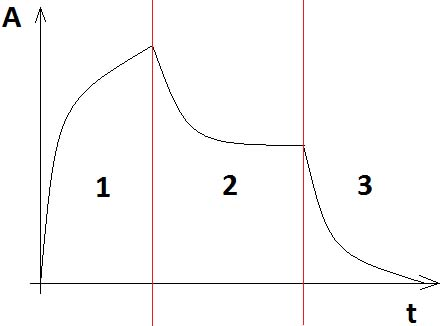
\epsfig{file=envA, scale=0.40}
      \caption{Example of envelope}
      \label{fig:envA}
    \end{center}
  \end{minipage}
  \hfill
  \begin{minipage}[t]{.45\textwidth}
    \begin{center}  
      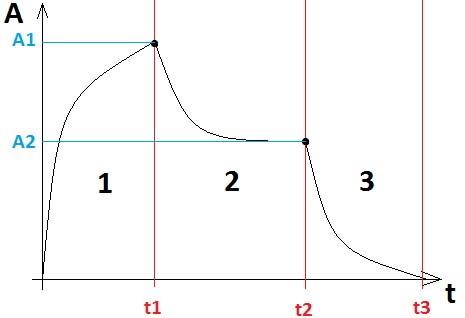
\epsfig{file=envB, scale=0.40}
      \caption{Envelope with the parameters for the equations}
      \label{fig:envB}
    \end{center}
  \end{minipage}
  \hfill
\end{figure}\\
There is also a fourth section but it is not shown in figure \ref{fig:envA}. This section is called "sustain". It is actually the section between the decay and the release. The reason it is not shown is because sustain time is not predetermined. The sustain lasts until, in the case of a synthesizer , a button is released after the attack and decay. Then the envelope passes into the release. The amplitude of the sustain is constant and is equal to the final amplitude of the decay.
%----------------------------------------------------------------------------------------
\subsection{Mathematical equations}
The attack, decay and release all have a different but similar equation, respectively equations \ref{eq:1}, \ref{eq:2} and \ref{eq:3}:
\begin{equation}
A = \frac{A_{1}}{t_{1}^{slope_{1}}} \cdot t^{slope_{1}}
\end{equation}
\begin{equation}
A = \frac{A_{2} - A_{1}}{ (t_{2} - t_{1})^{slope_{2}}} \cdot (t  -t_{1})^{slope_{2}} + A_{1}
\end{equation}
\begin{equation}
A = \frac{- A_{2}}{(t_{3} - t_{2})^{slope_{3}}} \cdot (t - t_{2})^{slope_{3}} + A_{2}
\end{equation}
The variables A1, A2, t1, t2 and t3 are represented in figure \ref{fig:envB}. Slope 1, slope2 and slope 3 are the slopes of section 1, 2 and 3 respectively. \\
Figure \ref{fig:slopes} shows examples of the attack with different slopes. The straight line in the middle is an attack with a slope of 1. If slope becomes larger than 1, the attack will rise first at a slow rate and then faster in an exponential way. The larger the slope, the faster the attack will rise at the end. If the slope is larger than 0 but smaller than 1, the attack will first rise fast and then slower in an exponential way.
\begin{figure}[htbp]
\centering
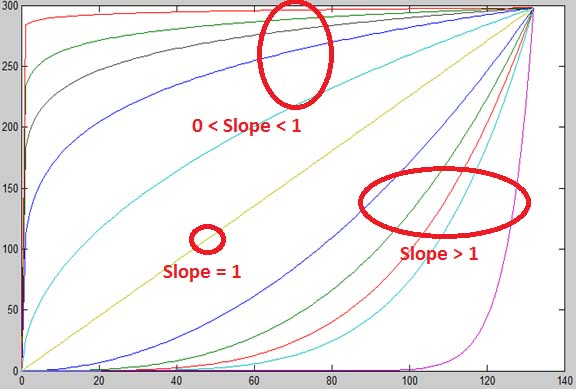
\includegraphics[height=6cm]{envC}
\rule{30em}{0.5pt}
\caption{Different slopes for the attack}
\label{fig:slopes}
\end{figure}
%----------------------------------------------------------------------------------------
\subsection{Envelopes and modulation}
When modulating a signal, only the carrier is hearable (Bjorn does not agree with this!). With an envelope you can make a sound for example fade in or out. The modulators only change the original (carrier) signal but the modulators aren't directly hearable.\\  
The modulators, however, do have an envelope as well. We know that when we modulate a signal, the modulation is also dependent on the modulation index ''I". This value is an indication for how hard the original signal gets modulated. The envelope of the modulators change the value ''I". In this way a modulation is affected by the envelope.
%----------------------------------------------------------------------------------------
\subsection{Envelopes in the program}
Each operator has a variable" envEn"(Bool), "time"(int) and "count"(int). The parameter envEn is a boolean and it is used to switch the envelopes on or off. While modulating (Bjorn: also without modulation), the program checks if envEn is true. If this is the case time increases by 1. If this is not the case time and count each become 0. If envEn is true and time is equal to the sampling frequency (96000Hz), count increases by one. This is to indicate that a period of 1 second has elapsed. \\
Below is the algorithm for the envelopes shown. The variable "totTime" is the total time of the envelope. The program checks if the envelopes are enabled. If this is true, it checks if the totTime
 $<=$ endPointATKt, $>$ endPointATKt and $<=$ endPointDECt or $>$ endPointRELt. This is a way for the program to know in which phase of the envelope totTime is located (attack, decay or release). If totTime is greater than endPointRELt, the variable envEn becomes false so the envelope will repeat itself as long as the user doesn't turn off the envelopes.
If the envelopes are not enabled, the amplitude of the wave is constant and equal to the amplitude the user chose on the interface. 
\begin{alltt}
for(i=0; i<4; i++)
{
   (op[i].envEn == TRUE) ? (op[i].env.time)++ : (op[i].env.time = op[i].env.count = 0);
   if(op[i].envEn == TRUE && !(op[i].env.time%=sampleFreq)) op[i].env.count++;
}

if(op->envEn)
{
   totTime = op->env.time + op->env.count * sampleFreq;	

   if(totTime <= endPointATKt)
      result=(op->amplitude/(powf(endPointATKt,slope1)))*powf(totTime,slope1);
   else if(totTime > endPointATKt && totTime <= endPointDECt)
      result=((((endPointDECa - op->amplitude)/powf((endPointDECt - endPointATKt),slope2)) 
             *powf((totTime - endPointATKt),slope2)) + op->amplitude);
   else if(totTime > endPointDECt && totTime <= endPointRELt)
      result=(((-endPointDECa/powf((endPointRELt-endPointDECt),slope3))*powf((totTime 
             - endPointDECt),slope3)) + endPointDECa);
   else if(totTime > endPointRELt)
      op->envEn = FALSE;			
}
else  result = op->amplitude;

return result;
\end{alltt}
%----------------------------------------------------------------------------------------
\subsection{Problems that occurred during the course of the project}
There were a lot of problems with the envelopes. At first there was only one variable time for all the operators. This way the envelopes worked too but it was confusing to program with and the envelope would not start from the beginning. It was also not possible to make the envelopes repeat properly without individual timers for each operator (Bjorn: not true!). \\
Another problem was the variable count. At first count would not increase of each operator individually. The counts of all enabled envelopes would increase at the same time when time\%=96000 would equal to 0. The problem that would occur was that count would only increase every 4 seconds instead of 1. Every time a block of 1024 samples is processed, time increases by 1024. This, however, would cause time\%=96000 to be only 0 when time reached 384000 which is equal to 96000*4.\\
To solve this problem we would let the counts of the enabled envelopes increase in the function "createSignal" itself. The function \verb+updateEnvelopes()+ increases the counts of all enabled envelopes. Now count would increase properly every second. Another problem occurred when modulating. If we for example modulate with 2 operators. If time would become 96000, count of operator 1 and operator 2 would both increase. If the envelope of the first operator would then be calculated there would be no problem. The problem would occur with the second operator. Count of this operator would have increased at the same time as count of the first operator. This would cause the envelope of the second operator to skip samples because totTime of that envelope would not have the right value. This problem could be solved by making the counts of the enabled envelopes increase individually. 
\begin{alltt}
void createSignal(Operator *op, int t)
{
   int i;
   float scalar;
   scalar=powf(2.0,23.0);
   switch(op->wave)
   {	
   case SINE:
      for(i=0; i<NUM_SAMPLES; i++)
      {
            op->signal[i] = envelope(op, &t)*sin( 2.0 * 3.141592 * 
                                            op->frequency / sampleFreq * t );
            t+= 1;
            if(!(t\%=sampleFreq)) updateEnvelopes(); //nrT++
            t\%=sampleFreq;
      }
      break;
	}
}
\end{alltt}
\begin{remark}
Please see the section ''Key functions'' \ref{code:createSignal} for the correct version of this function and without unused variables and double operations.
\end{remark}
%----------------------------------------------------------------------------------------
\section{Keyboard control}
The synthesizer must be able to play different music notes with the press of a key on the keyboard like a piano.\\ 
Figure \ref{fig:piano} shows the labview algorithm for keyboard control of the synthesizer. This sample algorithm checks if "B" on the keyboard is pressed. In short these are the steps the program goes through to accomplish this: 
\begin{enumerate}
\item The algorithm first checks if the Boolean to switch on the keyboard is true. If this is the case, the algorithm goes to step 2 (this step is not shown on figure \ref{fig:piano1}).
\item The pressed key gets registered by the program. On figure \ref{fig:piano1} the keyboard is shown with all the buttons.
\item The name of the pressed key is stored in an array and the pressed keys on the keyboard interface get a darker color as long as the keys are pressed. Labview assumes you are using a QWERTY keyboard so in figure 2 the requirement is "Z" but on an AZERTY keyboard this is "W". The user doesn't have to know this because he/she only has to look at the interface of the keyboard.
\item The case structure checks if the name of the key is equal to "Z" in this case.
\item If the key is pressed: The associated key on the interface becomes darker and the frequency of the sound that gets created becomes 31Hz in this case. The frequencies of the other buttons are $2^{\frac{1}{12}}$ times the frequency of the previous one. For example, the frequency of "S" is $2^{\frac{1}{12}}$ times the frequency of "W" and the frequency of "X" is $2^{\frac{1}{12}}$ times the frequency of "S".
If no key is pressed: frequency of the sound automatically becomes 0.
\item The while loop repeats.
\end{enumerate}
We made 2 octaves of buttons for the interface which means that every button in the second octave has a frequency that is twice the frequency of the corresponding button on the first octave.
\begin{figure}[htbp]
\centering
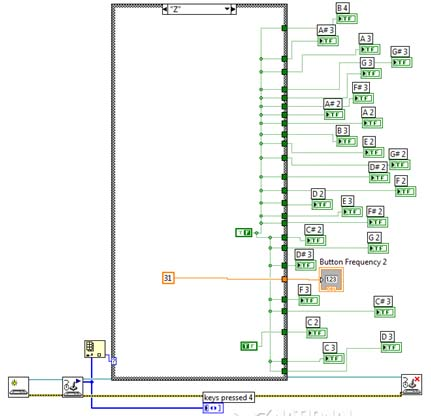
\includegraphics[height=10cm]{piano}
\rule{30em}{0.5pt}
\caption{Labview algorithm for keyboard control}
\label{fig:piano}
\end{figure} \\
\begin{figure}[htbp]
\centering
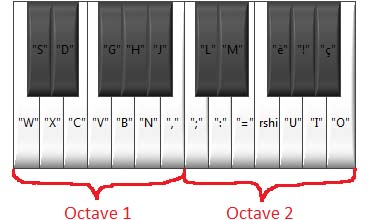
\includegraphics[height=5cm]{piano1}
\rule{30em}{0.5pt}
\caption{Keyboard buttons}
\label{fig:piano1}
\end{figure} 
